\documentclass[a4paper, 12pt]{article}
\usepackage[a4paper,top=1.5cm, bottom=1.5cm, left=1cm, right=1cm]{geometry}
\usepackage{cmap}					% поиск в PDF
\usepackage{mathtext} 				% русские буквы в формулах
\usepackage[T2A]{fontenc}			% кодировка
\usepackage[utf8]{inputenc}			% кодировка исходного текста
\usepackage[english,russian]{babel}	% локализация и переносы

\usepackage{amsmath,amssymb}
\usepackage{indentfirst}
\usepackage{longtable}
\usepackage{graphicx}
\usepackage{array}
\usepackage{float}

\usepackage{floatflt}
\usepackage{wrapfig}
\usepackage{siunitx} % Required for alignment
\usepackage{subfigure}
\usepackage{multirow}
\usepackage{rotating}
\usepackage{caption}

\graphicspath{{.}}


\title{\begin{center}Лабораторная работа №3.4.1\end{center}
Диа- и парамагнетики}
\author{Рожков А. В.}
\date{\today}

\begin{document}
    \pagenumbering{gobble}
    \maketitle
    \newpage
    \pagenumbering{arabic}

    \textbf{Цель работы:} измерение магнитной восприимчивости диа- и парамагнитных образцов.

    \textbf{В работе используются:} электромагнит, аналитические весы, милливеберметр, регулируемый источник постоянного тока, образцы.

    \section{Теоретическая справка}

        Магнитная восприимчивость тел может быть определена по измерению сил, действующих на тела в магнитном поле. Одним из классических методов таких измерений является т.н. \textit{метод Гюи}. В нём используется длинный тонкий стержень, один из концов которого помещают в зазор электромагнита (обычно в область однородного поля), а другой конец -- вне зазора, где величиной магнитного поля можно пренебречь. В этом случае закон изменения поля -- от максимального до нулевого -- будет несущественен.

        Найдём выражение для силы, действующей со стороны магнитного поля на помещённый в зазор электромагнита цилиндрический стержень. Пусть площадь его сечения равна $S$, его магнитная проницаемость -- $\mu$, поле в зазоре -- $B_0$, а глубина, на которую стержень помещён в зазор, -- $x$. Так как ток $I$ через электромагнит остаётся постоянным, то сила, действующая на стержень со стороны магнитного поля, равна производной магнитной энергии системы по координате, взятой с противоположным знаком:\[F_M=\left(\frac{\partial W_M}{\partial x}\right)_I,\]где $W_M(x)$ -- магнитная энергия системы при $I=\text{const}$ (то есть при $B_0=\text{const}$) в зависимости от глубины погружения стержня $x$.

        Объёмную плотность магнитной энергии можно найти по формуле:\[W_M=\frac{1}{2\mu_0}\int\frac{B^2}{\mu}\text{d}V,\]где интеграл берётся по всему пространству.

        Найдём теперь распределение магнитного поля в цилиндре. Рассмотрим сначала бесконечный стержень с проницаемостью $\mu$, помещённый в перпендикулярное ему однородное поле $B_0=\mu_0H_0$, и найдём поле $B_{\text{ст}}$ внутри него. В силу малости магнитной восприимчивости исследуемых образцов можно воспользоваться непрерывностью касательной компоненты $H$ и считать, что внутри стержня $H_{\text{ст}}=H_0$, потому $B_{\text{ст}}=\mu B_0$. Тогда систему из стержня в зазоре электромагнита можно условно разбить на три части -- вне электромагнита (I), в погружённой части стержня (II) и в электромагните вдали от стержня (III). В области I поле мало ($B_1\approx0$), поэтому его вкладом в энергию можно пренебречь. В области II поле приближённо равно $B_2\approx\mu B_0$, а в области III -- $B_3\approx B_0$.

        При смещении цилиндра вглубь электромагнита на $\text{d}x$ область II увеличивается в объёме на $\text{d}V_2=S\text{d}x$, а область III уменьшается на $\text{d}V_3=-S\text{d}x$. Распределение поля в пограничных участках между областями при этом почти не меняется. Тогда изменение магнитной энергии при таком смещении равно:\[\text{d}W_M(\text{d}x)\approx\frac{B_2^2}{2\mu\mu_0}S\text{d}x-\frac{B_2^2}{2\mu_0}S\text{d}x=\left(\mu-1\right)\frac{B_0^2}{2\mu_0}S\text{d}x.\]Следовательно, искомая сила равна:\[F_M=\left(\frac{\partial W_M}{\partial x}\right)_{B_0}\approx\chi\frac{B_0^2}{2\mu_0}S.\]

        Знак силы зависит от знака восприимчивости $\chi=\mu-1$: парамагнетики ($\chi > 0$) \textit{втягиваются} в зазор электромагнита, а диамагнетики ($\chi < 0$) \textit{выталкиваются} из него. Таким образом, измерив силу, действующую на образец в магнитном поле $B_0$, можно рассчитать его магнитную восприимчивость.

    \section{Экспериментальная установка}

        Схема установки показана на рисунке \ref{img:device}. Магнитное поле с максимальной индукцией $\approx1~\text{Тл}$ создаётся в зазоре электромагнита, питаемого постоянным током. Диаметр его полюсов существенно превосходит ширину зазора, поэтому поле в его средней части достаточно однородно. Величина тока, проходящего через обмотки электромагнита, задаётся регулируемым источником постоянного тока.

        \begin{figure}[h]
            \centering
            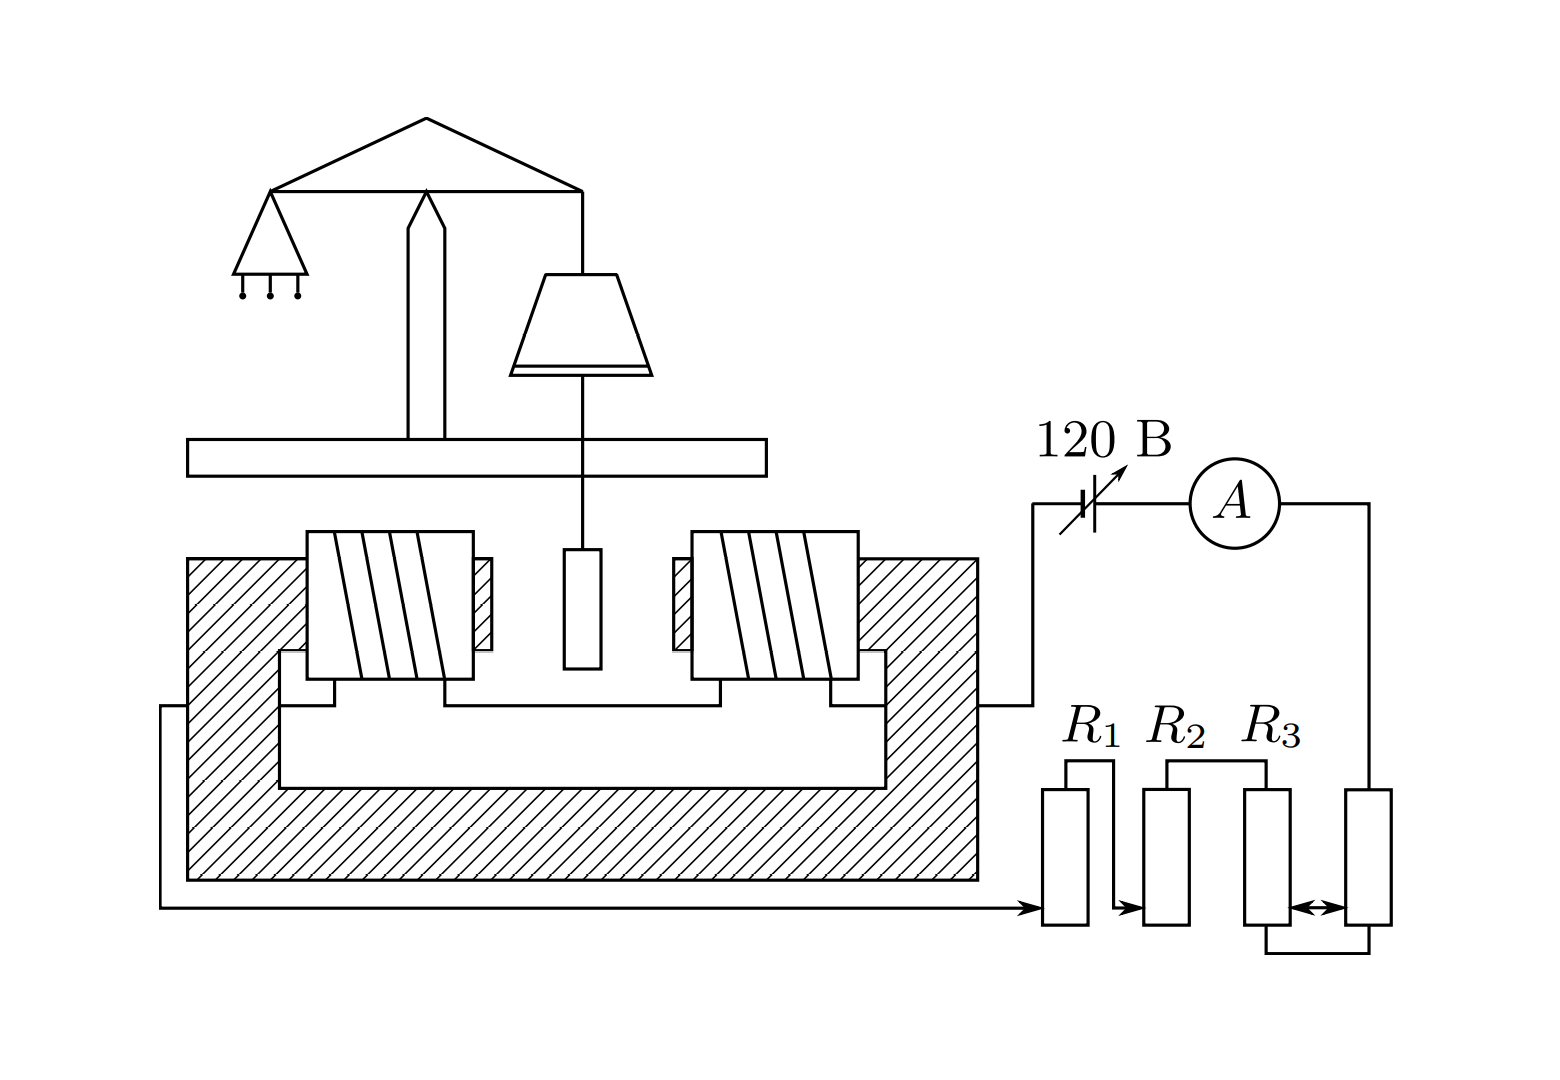
\includegraphics[scale=0.35]{img/device.png}
            \caption{Схема экспериментальной установки} \label{img:device}
        \end{figure}

        Градуировка электромагнита (связь между индукцией магнитного поля $B$ в зазоре и силой тока $I$ в обмотках) производится при помощи милливеберметра. При измерениях образцы поочерёдно подвешиваются к аналитическим весам так, что один конец образца оказывается в зазоре электромагнита, а другой -- вне его, где индукцией магнитного поля можно пренебречь. При помощи аналитических весов определяется перегрузка $\Delta P=F$ -- сила, действующая на образец со стороны магнитного поля.

        Погрешности приборов: милливеберметра -- половина цены деления шкалы, т.е. $\Delta\Phi=0.05~\text{мВб}$, электрических приборов -- амперметра и весов -- $0,5\%+2~\text{ед. мл. разряда}$.

    \section{Ход работы}

        \subsection{Градуировка электромагнита}

            При помощи милливеберметра построим градуировочную кривую $B(I)$.

            \begin{figure}[h]
                \centering
                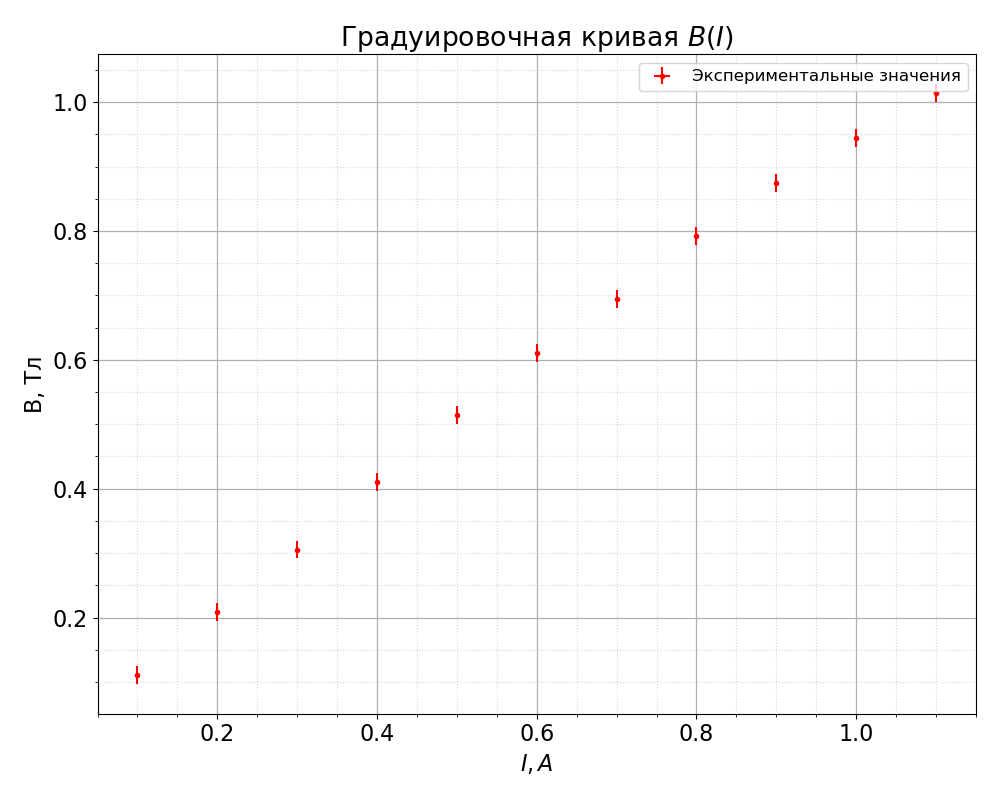
\includegraphics[scale=0.5]{img/grad.png}
                \caption{градуировочная кривая $B(I)$} \label{img:grad}
            \end{figure}

        \subsection{Измерения для меди и алюминия}

            Построим графики $\Delta P = f(B^2)$. По наклонам определим магнитную восприимчивость $\chi$.

            \begin{figure}[h]
                \centering
                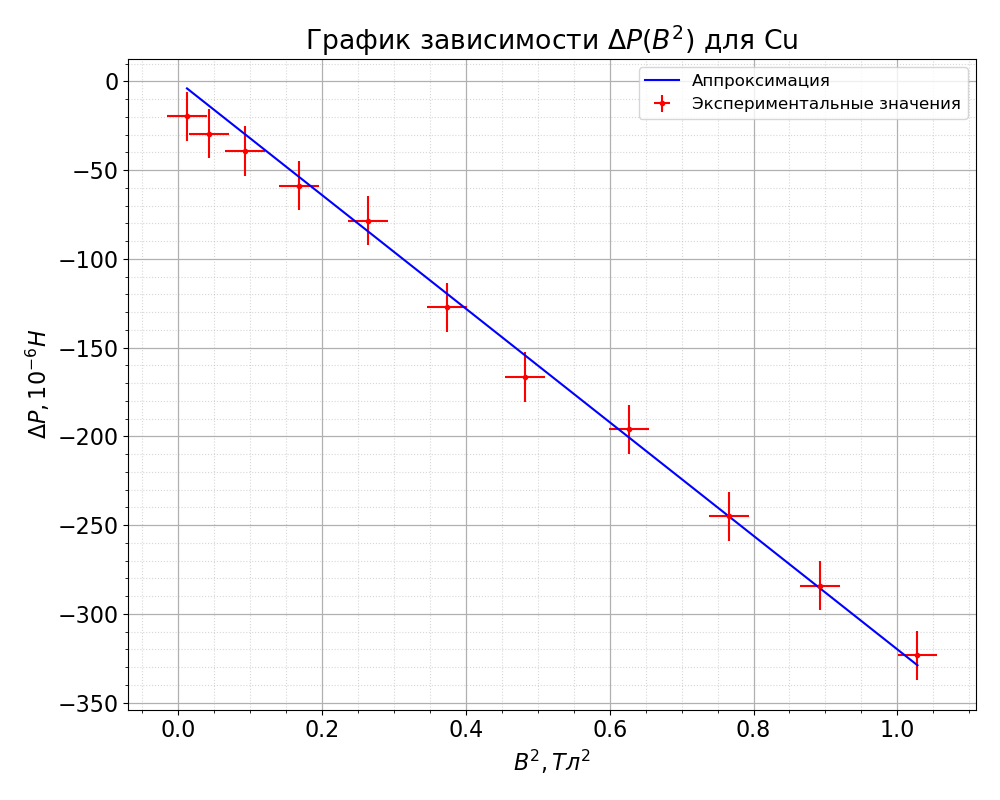
\includegraphics[scale=0.5]{img/Cu.png}
                \caption{График $\Delta P = f(B^2)$ для меди} \label{img:Cu}
            \end{figure}

            \begin{figure}[h]
                \centering
                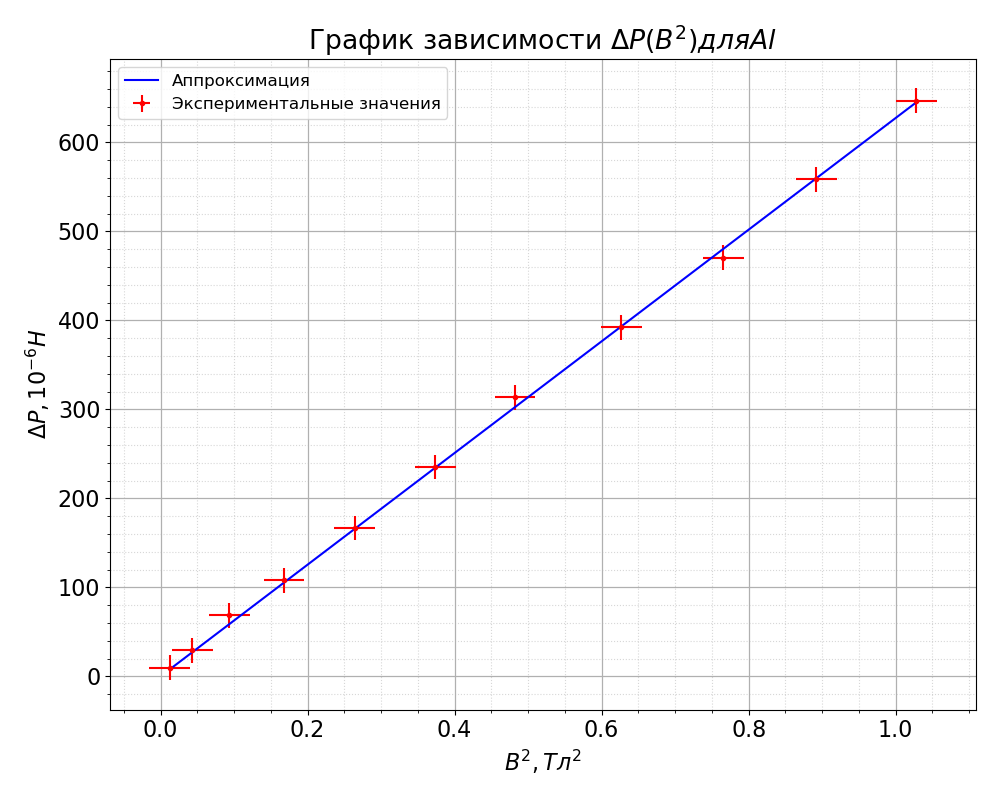
\includegraphics[scale=0.5]{img/Al.png}
                \caption{График $\Delta P = f(B^2)$ для алюминия} \label{img:Al}
            \end{figure}

            \begin{table}[!ht]
                \centering
                \begin{tabular}{|c|c|c|}
                    \hline

                    Материал & $\chi, 10^{-5}$ & $\chi_{табл}, 10^{-5}$\\ \hline
                    Cu & $-1.02 \pm 0.02$ & -0.92\\ \hline
                    Al & $2.008 \pm 0.010$ & 2.3\\ \hline

                \end{tabular}
                \caption{Результаты}
                \label{tab:res}
            \end{table}

    \section{Вывод}
        С помощью метода Гюи мы измерили магнитную восприимчивость меди и алюминия и поняли, что медь диамагнетик, а алюминий парамагнетик. Значения магнитной восприимчивости достаточно близки к табличным.

\end{document}
